The following games appear in books from the $1950$s and $60$s, where they were used as demonstrations that the solutions of continuous games may be supported on anything from singleton sets to Cantor sets and whole intervals.

\begin{game}\label{ex.dresher61.pg110}
A two-player zero-sum game in $1 \times 1$ variables on the interval
$$x_{i1} \in [0,1] \quad \forall i \in \{1, 2\},$$
with the utility function \cite[pg. 110]{Dresher2007-ez}
\begin{equation*}
u_{1}\left( x_{1}, x_{2} \right) = \left( x_{11} - x_{21} \right)^{2}
\end{equation*}
The Nash equilibrium is $\mu_1^\star = \mathcal{U}\{0,1\}$; $\mu_2^\star = \delta_{0.5}$ and the value is $\frac{1}{4}$.
\end{game}

\noindent
\begin{minipage}[c]{0.6\textwidth}
\begin{game}\label{ex.dresher61.pg111}
A two-player zero-sum game in $1 \times 1$ variables on the interval
$$x_{i1} \in [0,1] \quad \forall i \in \{1, 2\},$$
with the utility function
\begin{align*}
u_{1}\left( x_{1}, x_{2} \right) &= \left( 1 - \left| x_{21} - x_{11} \right| \right) \left|  x_{21} - x_{11} \right|
\end{align*}
\textcite[pg. 111]{Dresher2007-ez} proved that the only equilibrium of this game has an infinite support: $\mu_i^\star = \mathcal{U}[0,1]$, and its value is $\frac{1}{6}$.
\end{game}
\end{minipage}
\hfill
\begin{minipage}[c]{0.35\textwidth}
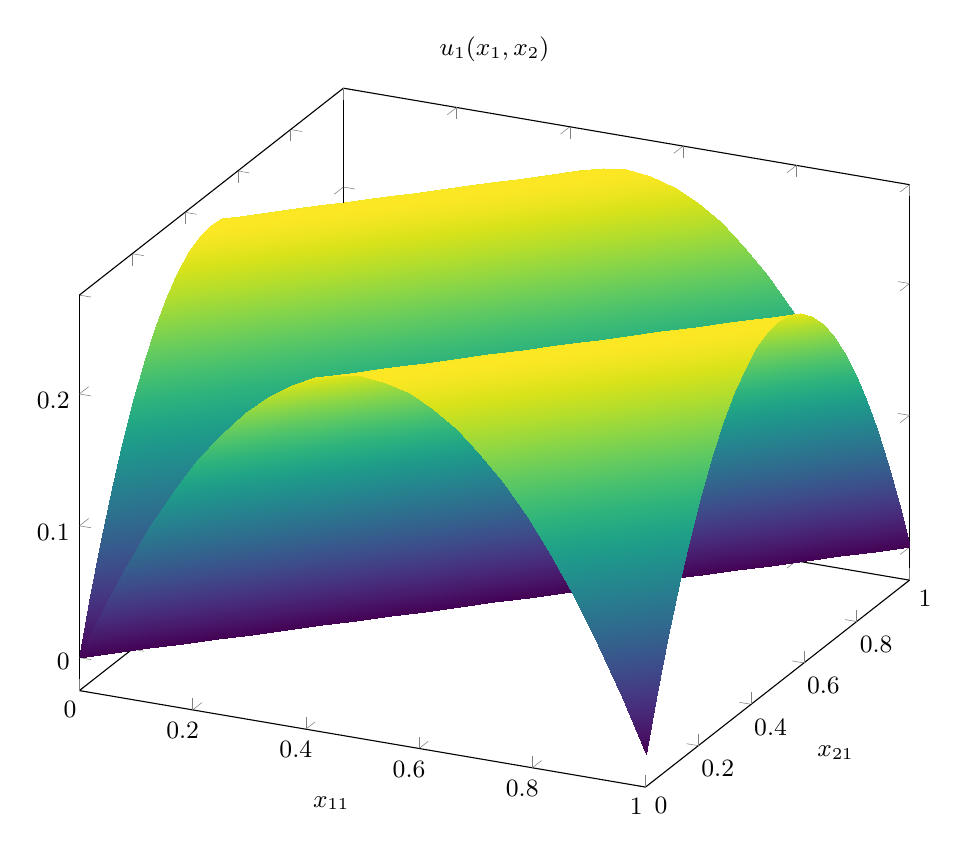
\begin{tikzpicture}
\begin{axis}[
    font=\small,
    domain=0:1,
    y domain=0:1,
    xlabel=$x_{11}$,
    ylabel=$x_{21}$,
    title={$u_1(x_1,x_2)$},
    colormap/viridis,
    mesh/ordering=y varies,
    width=\textwidth,
]
\addplot3[
    surf,
    shader=interp,
]
{abs(y - x) * (1 - abs(y - x))};
\end{axis}
\end{tikzpicture}
\end{minipage}


\begin{game} \label{ex.gross58.poly}
A two-player zero-sum game in $m_1 \times m_2$ variables on compact subsets of real numbers
\[
    x_i \in X_i \subset \mathbb{R}^{m_i} \quad \forall i \in \{1,2\}.
\]
The polynomial utility function is defined by
\begin{align*}
u(x_1,x_2)
= &f(x_1)ϕ(x_1) \left(g(x_2)ϕ(x_1) + \sum_{i=1}^{c_2} (g_i(x_2) - \mu_{2i}) ϕ_i(x_1) \right) \\
- &g(x_2)ψ(x_2) \left(f(x_1)ψ(x_2) + \sum_{i=1}^{c_1} (f_i(x_1) - \mu_{1i}) ψ_i(x_2) \right) \\
- &(f(x_1)ϕ(x_1))^2 + (g(x_2)ψ(x_2))^2
\end{align*}
where
\begin{align*}
f(x_1) &= \prod_{\substack{s \in \sigma_1}} \norm{x_1 - s}^2, &\phi(x_1) &= \prod_{\substack{a \in \alpha_1}} \norm{x_1 - a}^2,\\
f_i(x_1) &= \prod_{\substack{s \in \sigma_1 \\ s \neq \sigma_{1i}}} \frac{\norm{z-s}^2}{\norm{\sigma_{1i}-s}^2},&\phi_i(x_1) &= \prod_{\substack{a \in \alpha_1 \\ a \neq \alpha_{1i}}} \norm{x_1-a}^2;
\end{align*}
with $g$ and $\psi$ being defined analogously for $x_2$, $\sigma_2$, $\mu_2$, and $\alpha_2$.

This game has the property that the parameters $\sigma$ and $\mu$ define a unique mixed Nash equilibrium supported on $\sigma_i \in X_i^{c_i}$ weighted by $\mu_i \in \Delta^{c_i-1}$, for any set of cluster points $\alpha_i \in X_i^{c_{-i}+1}$ that do not overlap with the supports.

This construction of polynomial games with a unique prescribed solution was discovered by \textcite{gale1958note}. The generated games may be challenging to solve numerically given their large degrees and relative flatness near the equilibrium as shown in figure \ref{fig:gross}.
\end{game}

\begin{figure}
\centering
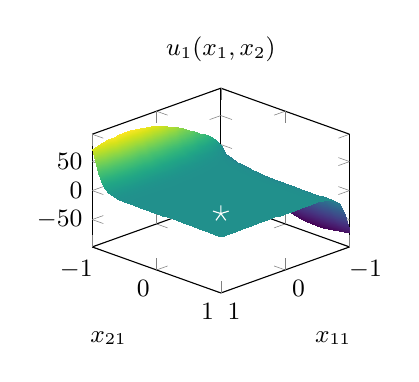
\begin{tikzpicture}
\begin{axis}[
    font=\small,
    domain=-1:1,
    y domain=-1:1,
    xlabel=$x_{11}$,
    ylabel=$x_{21}$,
    title={$u_1(x_1,x_2)$},
    colormap/viridis,
    view={135}{30},
    mesh/ordering=y varies,
    width=0.4\textwidth,
]
\addplot3[
    surf,
    shader=interp,
]
{-0.25*y^5 + 0.25*x*y^4 - 0.25*x^4*y + 0.25*x^5 + 2.25*y^6 - 2.0*x*y^5 - 0.25*x^2*y^4 + 0.25*x^4*y^2 + 2.0*x^5*y - 2.25*x^6 - 8.5*y^7 + 6.5*x*y^6 + 2.0*x^2*y^5 - 2.0*x^5*y^2 - 6.5*x^6*y + 8.5*x^7 + 17.5*y^8 - 11.0*x*y^7 - 6.5*x^2*y^6 + 6.5*x^6*y^2 + 11.0*x^7*y - 17.5*x^8 - 21.25*y^9 + 10.25*x*y^8 + 11.0*x^2*y^7 - 11.0*x^7*y^2 - 10.25*x^8*y + 21.25*x^9 + 15.25*y^10 - 5.0*x*y^9 - 10.25*x^2*y^8 + 10.25*x^8*y^2 + 5.0*x^9*y - 15.25*x^10 - 6.0*y^11 + x*y^10 + 5.0*x^2*y^9 - 5.0*x^9*y^2 - x^10*y + 6.0*x^11 + y^12 - x^2*y^10 + x^10*y^2 - x^12};
\addplot3[
    only marks,
    mark=star,
    color=white,
    mark size=3,
]
coordinates {(0.5, 0.5, 0)};
\end{axis}
\end{tikzpicture}
\caption{12-degree polynomial game on a hypercube with a prescribed solution at $0.5, 0.5$ constructed using the method described by \textcite{gale1958note}  with parameters $\alpha_i = (1, 0)$, $\sigma_i = (0.5)$, and $\mu_i = (1) \quad \forall i \in \{1,2\}$.}
\label{fig:gross}
\end{figure}

\begin{game}\label{ex.karlin59.vol2.sec71.ex1}
A two-player zero-sum game in $1 \times 1$ variables on the interval
$$x_{i1} \in [0,1] \quad \forall i \in \{1,2\}.$$
The utility function is defined by
\begin{equation*}
u_{1}\left( x_{1}, x_{2} \right) = \frac{1}{1 + \lambda \left( x_{11} - x_{21} \right)^{2}}
\end{equation*}
where $\lambda > 0$. \textcite[Example~1]{karlin:chapter} proved that the game has finitely supported optimal strategies.
\end{game}


\noindent
\begin{minipage}[c]{0.6\textwidth}
\begin{game}\label{ex.karlin59.vol2.sec71.ex2}
A two-player zero-sum game in $1 \times 1$ variables on the interval
$$x_{i1} \in [0,1] \quad \forall i \in \{1,2\}.$$
The utility is defined by the rational function
\begin{align*}
u_{1}\left( x_{1}, x_{2} \right) &=  \left( x_{21} - 0.5 \right)\left(\frac{1 + \left( x_{21} - 0.5 \right)^{2} \left( x_{11} - 0.5 \right)}{1 + \left( x_{21} - 0.5 \right)^{4} \left( x_{11} - 0.5 \right)^{2}} \right) \\
& - \frac{x_{21} - 0.5 }{1 + \left( x_{21} - 0.5 \right)^{4} \left( \frac{1}{3} x_{11} -0.5\right)}
\end{align*}
\textcite[Example~2]{karlin:chapter} proved that the unique optimal strategy is the Cantor distribution.
\end{game}
\strut
\end{minipage}
\hfill
\begin{minipage}[c]{0.35\textwidth}
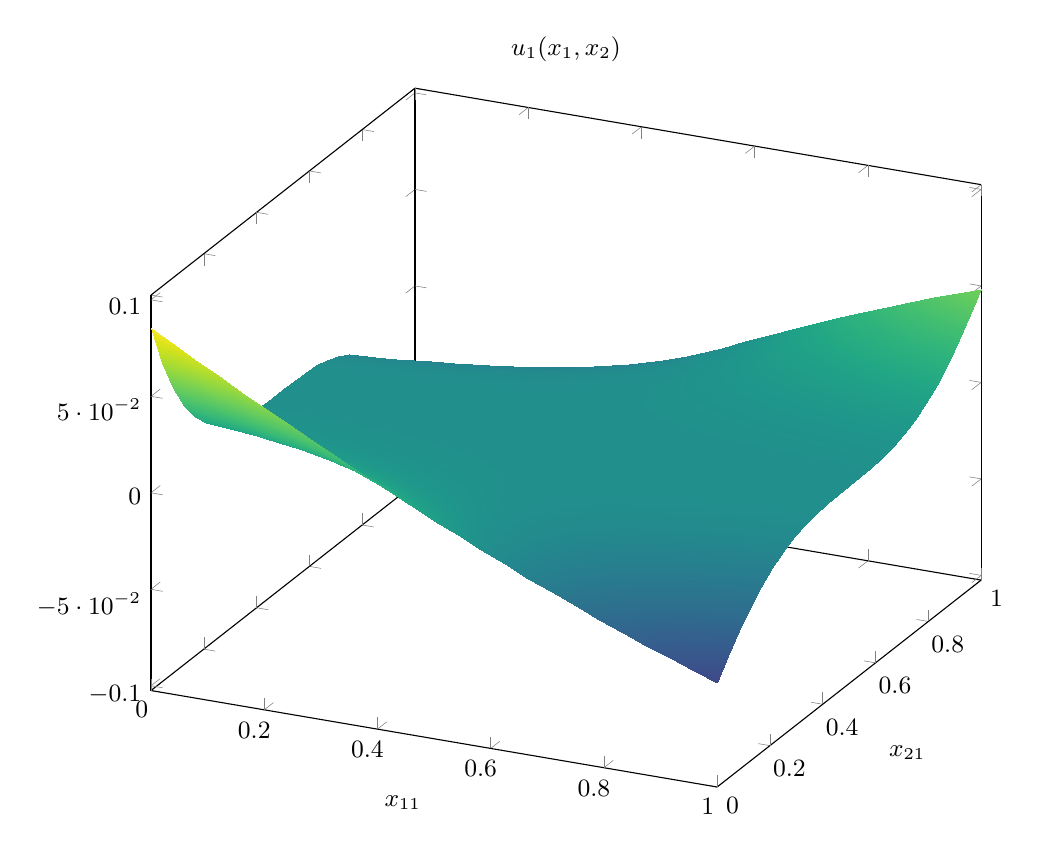
\begin{tikzpicture}
\begin{axis}[
    font=\small,
    domain=0:1,
    y domain=0:1,
    xlabel=$x_{11}$,
    ylabel=$x_{21}$,
    title={$u_1(x_1,x_2)$},
    colormap/viridis,
    mesh/ordering=y varies,
    width=\textwidth,
]
\addplot3[
    surf,
    shader=interp,
]
{(y - 0.5) * ((1 + (x - 0.5) * (y - 0.5)^2) / (1 + (x - 0.5)^2 * (y - 0.5)^4) - 1 / (1 + (x / 3 - 0.5) * (y - 0.5)^4))};
\end{axis}
\end{tikzpicture}
\end{minipage}


\begin{game}\label{ex.karlin59.vol2.sec76.pr1}
A two-player zero-sum game in $1 \times 1$ variables on the interval
$$x_{i1} \in [0,1] \quad \forall i \in \{1,2\}.$$
The utility is defined by \cite[Problem 1]{karlin:chapter}:
\begin{equation*}
u_{1}\left( x_{1}, x_{2} \right) = \frac{2 \left( x_{11} + x_{21} \right)}{\left( 1 + 2 x_{11} \right) \left( 1 + 2 x_{21} \right)}
\end{equation*}
The game has a Nash equilibrium where both players play $\mu^\star(z)=\frac{1+2z}{2}$.
\end{game}


\begin{game}\label{ex.karlin59.vol2.sec76.pr2}
A two-player zero-sum game in $1 \times 1$ variables on the interval
$$x_{i1} \in [0,1] \quad \forall i \in \{1,2\}.$$
The utility is defined by
\begin{equation*}
u_{1}\left( x_{1}, x_{2} \right) = \frac{\left( 1 + x_{11} \right) \left( 1 + x_{21} \right)}{\left( 1 + x_{11} x_{21} \right)^{2}}
\end{equation*}
\textcite[Problem 2]{karlin:chapter} showed that the value of this game is $\frac{1}{\ln 2}$ when both players play $\mu^\star(z)=\frac{\ln (1+z)}{\ln 2}$.

\end{game}

